\documentclass[12pt,a4paper]{article}

\usepackage[utf8]{inputenc}
\usepackage[spanish]{babel}
\usepackage[top=2.5cm,bottom=2.5cm,left=3cm,right=2.5cm]{geometry}
\usepackage{times}
\usepackage{setspace}
\usepackage{graphicx}
\usepackage{float}
\usepackage{booktabs}
\usepackage{array}
\usepackage{longtable}
\usepackage{xcolor}
\usepackage{enumitem}
\usepackage{amsmath}
\usepackage{fancyhdr}
\usepackage{hyperref}
\usepackage{caption}
\usepackage{pgfplots}
\usepackage{tikz}

\usetikzlibrary{babel,arrows.meta,positioning,shapes.geometric}
\pgfplotsset{compat=1.18}
\graphicspath{{../capturas/}{./}}
\onehalfspacing
\setlength{\parindent}{1.2cm}
\setlength{\parskip}{0.2cm}
\setlength{\tabcolsep}{5pt}

\definecolor{azulPuno}{HTML}{1B4F8A}
\definecolor{verdeSalud}{HTML}{2E7D32}
\definecolor{grisTexto}{HTML}{1F2937}
\definecolor{grisClaro}{HTML}{EEF3F7}

\hypersetup{
  colorlinks=true,
  linkcolor=azulPuno,
  urlcolor=azulPuno
}

\pagestyle{fancy}
\setlength{\headheight}{15pt}
\fancyhf{}
\lhead{UNAP}
\rhead{Informe de curso}
\cfoot{\thepage}

\begin{document}
\hypersetup{pageanchor=false}

\begin{titlepage}
\thispagestyle{empty}
\centering
\begin{minipage}{0.22\textwidth}
\centering

\includegraphics[height=2.5cm]{logo_unap.png}
\end{minipage}
\hfill
\begin{minipage}{0.52\textwidth}
\centering
{\Large\bfseries Universidad Nacional del Altiplano\par}
\vspace{0.15cm}
{\large Facultad de Ingenieria Estadistica e Informatica\par}
{\large Escuela Profesional de Ingenieria de Sistemas\par}
\end{minipage}
\hfill
\begin{minipage}{0.22\textwidth}
\centering

\includegraphics[height=2.5cm]{logo_sistemas.png}
\end{minipage}

\vspace{0.8cm}
{\color{azulPuno}\rule{\textwidth}{1.2pt}\par}
\vspace{0.55cm}
{\Large\bfseries Curso: Sistemas de Recomendacion\par}
\vspace{0.5cm}
{\huge\bfseries Informe del Proyecto de Curso\par}
\vspace{0.35cm}
{\Large\bfseries Sistema de Recomendacion de Centros de Salud Preventiva para la Region Puno\par}
\vspace{0.55cm}
{\color{azulPuno}\rule{\textwidth}{1.2pt}\par}

\vspace{0.6cm}
\begin{tabular}{rl}
Area de aplicacion: & Salud preventiva \\
Enfoque: & Sistema de recomendacion basado en contenido \\
Region: & Puno, Peru \\
\end{tabular}

\vspace{0.55cm}
\begin{tabular}{rl}
Responsable de asignatura: & Gonzales Paco Magali Gianina \\
\end{tabular}

\vspace{0.65cm}
{\large\bfseries Integrantes\par}
\vspace{0.2cm}
\begin{tabular}{l}
Aracayo Mamani, Jhon Marco \\
Canaza Paucara, Juan Diego \\
Luque Pacheco, Angie Tatiana \\
\end{tabular}

\vfill
{\large Puno--Peru\par}
\end{titlepage}

\hypersetup{pageanchor=true}
\pagenumbering{roman}
\tableofcontents
\newpage
\pagenumbering{arabic}

\section{Introduccion}
Los sistemas de recomendacion permiten ordenar alternativas de acuerdo con las necesidades o caracteristicas de un usuario. En plataformas digitales se usan para sugerir peliculas, productos, cursos, noticias o musica. Sin embargo, la misma idea tambien puede aplicarse a problemas de interes social, siempre que el sistema sea claro, responsable y entendible para quien lo utiliza.

El proyecto desarrollado corresponde a un \textit{Sistema de Recomendacion de Centros de Salud Preventiva para la Region Puno}. La finalidad del prototipo es orientar al usuario hacia establecimientos de salud que puedan responder mejor a una necesidad preventiva, considerando el tipo de atencion solicitada, la ubicacion del usuario, la distancia maxima permitida y la condicion climatica del entorno.

La propuesta nace de una situacion realista. En Puno existen establecimientos de salud distribuidos en diferentes provincias y distritos. Para una persona que necesita vacunacion, control prenatal, control de crecimiento y desarrollo, tamizaje, nutricion, odontologia, psicologia o planificacion familiar, no siempre resulta suficiente conocer el establecimiento mas cercano. Tambien interesa saber si dicho establecimiento ofrece el servicio, si se encuentra dentro de un radio razonable y si las condiciones climaticas pueden afectar el traslado.

Por ese motivo, el sistema no fue disenado como un directorio simple. Un directorio muestra informacion, pero no prioriza. En cambio, un sistema de recomendacion compara alternativas y devuelve un ranking. En este caso, el ranking presenta los centros mas adecuados de acuerdo con los datos ingresados por el usuario. Asimismo, la interfaz explica el tipo de recomendacion utilizado y muestra razones de seleccion para que el resultado no parezca arbitrario.

El prototipo fue desarrollado como una aplicacion web completa. Incluye pantallas de presentacion, acceso, registro, consulta, resultados e historial. Tambien incluye un backend que procesa la informacion, una base de datos local para pruebas, un notebook de analisis y un informe tecnico complementario. De esta forma, el proyecto no se limita a una demostracion visual; integra datos, modelo, aplicacion y evidencias de funcionamiento.

\subsection{Proposito del informe}
El presente informe tiene como proposito describir de manera formal y completa el trabajo realizado para el curso de Sistemas de Recomendacion. A diferencia del informe tecnico, este documento esta orientado a explicar el proceso general del proyecto: que problema se abordo, como se trabajo la metodologia, como se construyo el recomendador, que resultados se obtuvieron y que evidencias respaldan el desarrollo.

El informe se organiza en cinco secciones principales: introduccion, metodologia, resultados, discusion y conclusiones. Ademas, se incluye un apartado final de evidencias, donde se registra el notebook, el informe tecnico, las capturas y una propuesta de sustentacion breve.

\subsection{Alcance del proyecto}
El alcance del proyecto es academico y funcional. El sistema puede ejecutarse localmente, generar recomendaciones y mostrar resultados reales dentro del prototipo. No se plantea como sistema oficial de salud ni reemplaza la confirmacion directa con el establecimiento. Su valor esta en demostrar la aplicacion de un sistema de recomendacion en un contexto regional y preventivo.

\section{Metodologia}
La metodologia se desarrollo en siete etapas: definicion del problema, identificacion de usuarios e items, recoleccion y preparacion de datos, analisis exploratorio, construccion del modelo de recomendacion, desarrollo de la aplicacion y validacion del prototipo. Esta organizacion permitio avanzar desde la idea inicial hasta una aplicacion funcional con evidencias.

\subsection{Etapa 1: Definicion del problema}
La primera decision fue elegir un dominio donde el uso de recomendaciones tenga sentido. Se selecciono salud preventiva porque el usuario necesita elegir entre varias alternativas posibles, y esa eleccion depende de mas de un criterio. En el contexto de Puno, una recomendacion debe considerar no solo la existencia del establecimiento, sino tambien la distancia, el servicio requerido y el clima.

El problema se definio de la siguiente forma: \textit{como recomendar centros de salud preventiva adecuados para un usuario de la region Puno, segun su ubicacion, tipo de atencion, distancia maxima y condiciones climaticas}. Esta formulacion permitio convertir una necesidad general en un problema tratable por un sistema de recomendacion.

\subsection{Etapa 2: Usuarios, items e interacciones}
En todo sistema de recomendacion es necesario identificar tres elementos: usuarios, items e interacciones. En el proyecto, los usuarios son personas que buscan orientacion para atencion preventiva. Los items son establecimientos de salud. Las interacciones son consultas preventivas realizadas desde la aplicacion.

\begin{table}[H]
\centering
\caption{Elementos principales del sistema de recomendacion.}
\label{tab:elementos}
\begin{tabular}{p{3.5cm}p{9cm}}
\toprule
Elemento & Definicion en el proyecto \\
\midrule
Usuario & Persona que necesita orientacion sobre un servicio preventivo. \\
Item & Establecimiento de salud candidato a ser recomendado. \\
Interaccion & Consulta ingresada por el usuario: servicio, edad, ubicacion, distancia y Top-N. \\
Contexto & Condiciones que influyen en la recomendacion, como distancia y clima. \\
Resultado & Ranking de centros recomendados, con explicacion visible para el usuario. \\
\bottomrule
\end{tabular}
\end{table}

La interaccion del usuario no se interpreta como una calificacion. Es decir, el sistema no pregunta si un centro tiene cinco estrellas o si le gusto al usuario. En esta primera version, la interaccion sirve para construir el perfil de busqueda y generar recomendaciones a partir de atributos del establecimiento.

\subsection{Etapa 3: Recoleccion y preparacion de datos}
La preparacion de datos fue una etapa central. El sistema necesita comparar establecimientos, por lo que cada centro debe contar con informacion organizada. Para el prototipo se considero un dataset reproducible con establecimientos de Puno, servicios preventivos, categoria, ubicacion, horario, capacidad aproximada y alerta climatica.

Los datos se organizaron en entidades. La entidad principal es el establecimiento de salud. Cada establecimiento puede tener varios servicios disponibles. Tambien se consideraron alertas climaticas, asociadas al territorio, para ajustar la conveniencia de la recomendacion.

\begin{table}[H]
\centering
\caption{Datos empleados en el prototipo.}
\label{tab:datos}
\small
\begin{tabular}{p{3.3cm}p{3.8cm}p{5.4cm}}
\toprule
Grupo de datos & Campo considerado & Uso dentro del sistema \\
\midrule
Establecimiento & Nombre & Identificacion visible en la interfaz. \\
Establecimiento & Categoria & Indicador de capacidad y complejidad. \\
Establecimiento & Latitud y longitud & Calculo de distancia frente al usuario. \\
Establecimiento & Horario & Informacion complementaria para la decision. \\
Servicio & Tipo de servicio & Comparacion con la atencion solicitada. \\
Clima & Nivel de alerta & Ajuste o penalidad del ranking. \\
Consulta & Servicio requerido & Construccion del perfil de recomendacion. \\
Consulta & Distancia maxima & Filtro territorial de candidatos. \\
\bottomrule
\end{tabular}
\end{table}

La limpieza de datos se concentro en normalizar nombres de servicios, revisar coordenadas, asegurar categorias coherentes y mantener solo establecimientos activos. Esta preparacion evita recomendaciones inconsistentes, por ejemplo sugerir un centro sin coordenadas validas o sin el servicio preventivo solicitado.

\subsection{Etapa 4: Analisis exploratorio}
El analisis exploratorio se realizo en el notebook. Se reviso la estructura del dataset, la cantidad de establecimientos, la distribucion por categorias, la disponibilidad de servicios y la representacion territorial. Este paso fue importante porque antes de recomendar es necesario conocer que informacion existe y que limitaciones presenta.

Tambien se observo que no todos los establecimientos ofrecen los mismos servicios. Esa diferencia justifica el uso de un recomendador: si todos los centros tuvieran exactamente los mismos atributos, bastaria con ordenar por distancia. Pero al existir variacion en servicios, categoria y clima, el ranking requiere combinar varios criterios.

\begin{figure}[H]
\centering
\begin{tikzpicture}
\begin{axis}[
    ybar,
    width=0.86\textwidth,
    height=7cm,
    bar width=18pt,
    ylabel={Cantidad referencial},
    symbolic x coords={I-1,I-2,I-3,I-4,II-1},
    xtick=data,
    ymin=0,
    ymax=5,
    nodes near coords,
    grid=major,
    grid style={gray!15}
]
\addplot[fill=azulPuno!75] coordinates {(I-1,1) (I-2,2) (I-3,2) (I-4,3) (II-1,2)};
\end{axis}
\end{tikzpicture}
\caption{Distribucion referencial de establecimientos por categoria.}
\label{fig:categorias}
\end{figure}

\subsection{Etapa 5: Construccion del recomendador}
El sistema utiliza un enfoque de recomendacion basado en contenido. Esto quiere decir que se recomienda a partir de las caracteristicas de los items. En el proyecto, un centro de salud es descrito por sus servicios, categoria, distancia, capacidad y condicion climatica. El usuario, por su parte, es representado por la consulta ingresada.

El proceso de recomendacion se resume asi:

\begin{enumerate}[leftmargin=*]
  \item El usuario ingresa el tipo de atencion preventiva que necesita.
  \item El sistema recibe su ubicacion y distancia maxima.
  \item Se filtran los establecimientos activos.
  \item Se calculan distancias aproximadas.
  \item Se comparan los servicios del establecimiento con la necesidad del usuario.
  \item Se ajusta el resultado considerando alerta climatica.
  \item Se ordenan los centros y se devuelve un ranking Top-N.
\end{enumerate}

\subsection{Etapa 6: Entrenamiento y ajuste del modelo}
En este proyecto no se realizo entrenamiento supervisado tradicional, porque no existen etiquetas historicas como ``usuario califico este centro con 5 estrellas''. En lugar de ello, se preparo un modelo basado en atributos. A este proceso se le puede entender como preparacion, ajuste y validacion de reglas de recomendacion.

El ajuste consistio en definir como representar los datos para que puedan compararse. Se construyeron vectores para el perfil de usuario y para cada establecimiento. Luego se uso similitud coseno para medir que tan cercano es un establecimiento respecto a la consulta. Finalmente, se aplico un ajuste por clima para que los centros en zonas con alerta no tengan la misma prioridad que los centros sin alerta.

La ventaja de este enfoque es que el sistema puede recomendar desde el inicio, incluso sin tener muchos usuarios registrados. Esta es una caracteristica importante para prototipos nuevos, donde todavia no existe historial suficiente para aplicar filtrado colaborativo.

\begin{table}[H]
\centering
\caption{Diferencia entre entrenamiento tradicional y ajuste realizado.}
\label{tab:entrenamiento}
\begin{tabular}{p{4.2cm}p{8.2cm}}
\toprule
Aspecto & Aplicacion en el proyecto \\
\midrule
Datos historicos & No se cuenta con ratings reales de usuarios. \\
Tipo de modelo & Basado en contenido y atributos de establecimientos. \\
Representacion & Vectores de usuario y de item. \\
Comparacion & Similitud entre la necesidad del usuario y cada centro. \\
Ajuste contextual & Penalidad por alerta climatica y filtro por distancia. \\
Resultado & Ranking Top-N de establecimientos recomendados. \\
\bottomrule
\end{tabular}
\end{table}

\subsection{Etapa 7: Desarrollo del sistema}
Luego de validar la logica de recomendacion en el notebook, se desarrollo la aplicacion. El backend se encarga de procesar las consultas y generar las recomendaciones. El frontend permite que el usuario interactue con el sistema mediante formularios, tarjetas, mapas y graficos.

\begin{figure}[H]
\centering
\begin{tikzpicture}[
  node distance=1.3cm,
  box/.style={rectangle, rounded corners, draw=azulPuno, fill=azulPuno!8, thick, minimum width=4.1cm, minimum height=0.95cm, align=center},
  arrow/.style={-Latex, thick, color=azulPuno}
]
\node[box] (user) {Usuario};
\node[box, below=of user] (front) {Interfaz web};
\node[box, below=of front] (api) {Servicio de recomendacion};
\node[box, below left=1.1cm and 0.7cm of api] (data) {Datos de salud\\y clima};
\node[box, below right=1.1cm and 0.7cm of api] (model) {Modelo basado\\en contenido};
\node[box, below=3cm of api] (rank) {Ranking de centros\\recomendados};
\draw[arrow] (user) -- (front);
\draw[arrow] (front) -- (api);
\draw[arrow] (api) -- (data);
\draw[arrow] (api) -- (model);
\draw[arrow] (data) -- (rank);
\draw[arrow] (model) -- (rank);
\end{tikzpicture}
\caption{Flujo general del prototipo implementado.}
\label{fig:flujo}
\end{figure}

\subsection{Etapa 8: Validacion}
La validacion se realizo mediante pruebas automatizadas y revision manual de la aplicacion. Se comprobaron los procesos de registro, inicio de sesion, generacion de recomendaciones e historial. Ademas, se compilo la interfaz para verificar que no existan errores de construccion.

\begin{table}[H]
\centering
\caption{Validaciones realizadas.}
\label{tab:validacion}
\begin{tabular}{p{4cm}p{7cm}p{2cm}}
\toprule
Componente & Validacion & Resultado \\
\midrule
Backend & Pruebas automatizadas de autenticacion y recomendacion. & Correcto \\
Modelo & Ordenamiento, similitud y penalidad climatica. & Correcto \\
Frontend & Compilacion y revision de pantallas. & Correcto \\
Flujo completo & Login, busqueda, resultados e historial. & Correcto \\
Evidencias & Capturas e informe tecnico. & Correcto \\
\bottomrule
\end{tabular}
\end{table}

\section{Resultados}
El resultado principal fue una aplicacion funcional capaz de generar recomendaciones de centros de salud preventiva. El sistema presenta un flujo completo desde el acceso hasta la revision del historial. La interfaz final muestra con claridad que se trata de un recomendador y no solo de una pagina informativa.

\subsection{Resultado funcional}
El usuario puede crear una cuenta o iniciar sesion con una cuenta de prueba. Despues accede al formulario de consulta preventiva, donde selecciona el servicio requerido, edad, ubicacion, distancia maxima y numero de recomendaciones. Con esos datos, el sistema devuelve un ranking con los establecimientos priorizados.

Cada recomendacion muestra informacion relevante: nombre del centro, categoria, distancia, horario, servicios disponibles, score final, similitud y penalidad climatica. Esta informacion ayuda a comprender la razon de cada resultado.

\subsection{Resultado visual}
La interfaz fue mejorada para ser mas formal, ordenada y adecuada al tema de salud preventiva. Se reemplazaron textos tecnicos por explicaciones orientadas al usuario. Por ejemplo, en la pantalla de acceso se muestra que el sistema utiliza recomendacion basada en contenido, similitud de criterios y ajuste territorial, en lugar de presentar conceptos internos que no aportan a la sustentacion.

\begin{figure}[H]
\centering
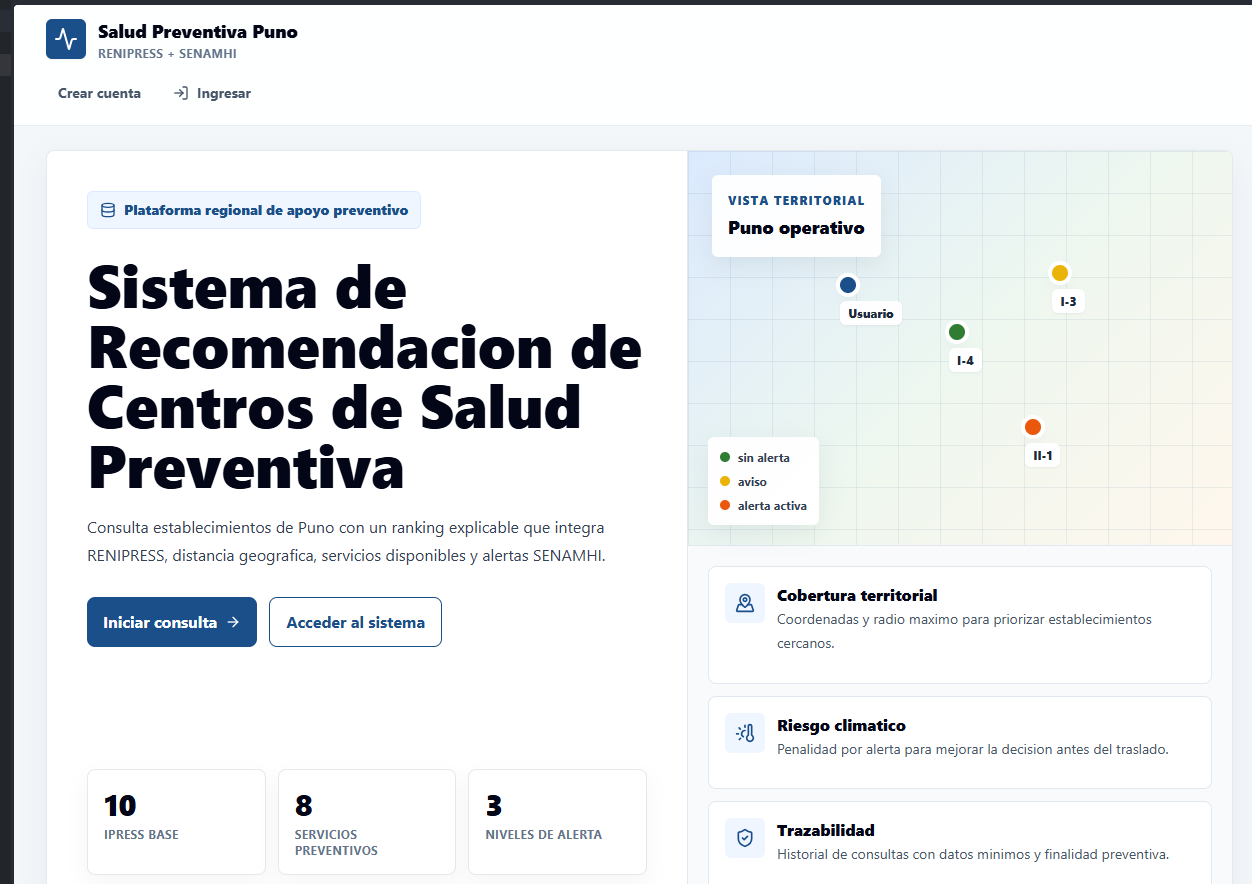
\includegraphics[width=0.92\textwidth]{landing.png}
\caption{Pantalla de presentacion del sistema.}
\label{fig:landing}
\end{figure}

\begin{figure}[H]
\centering
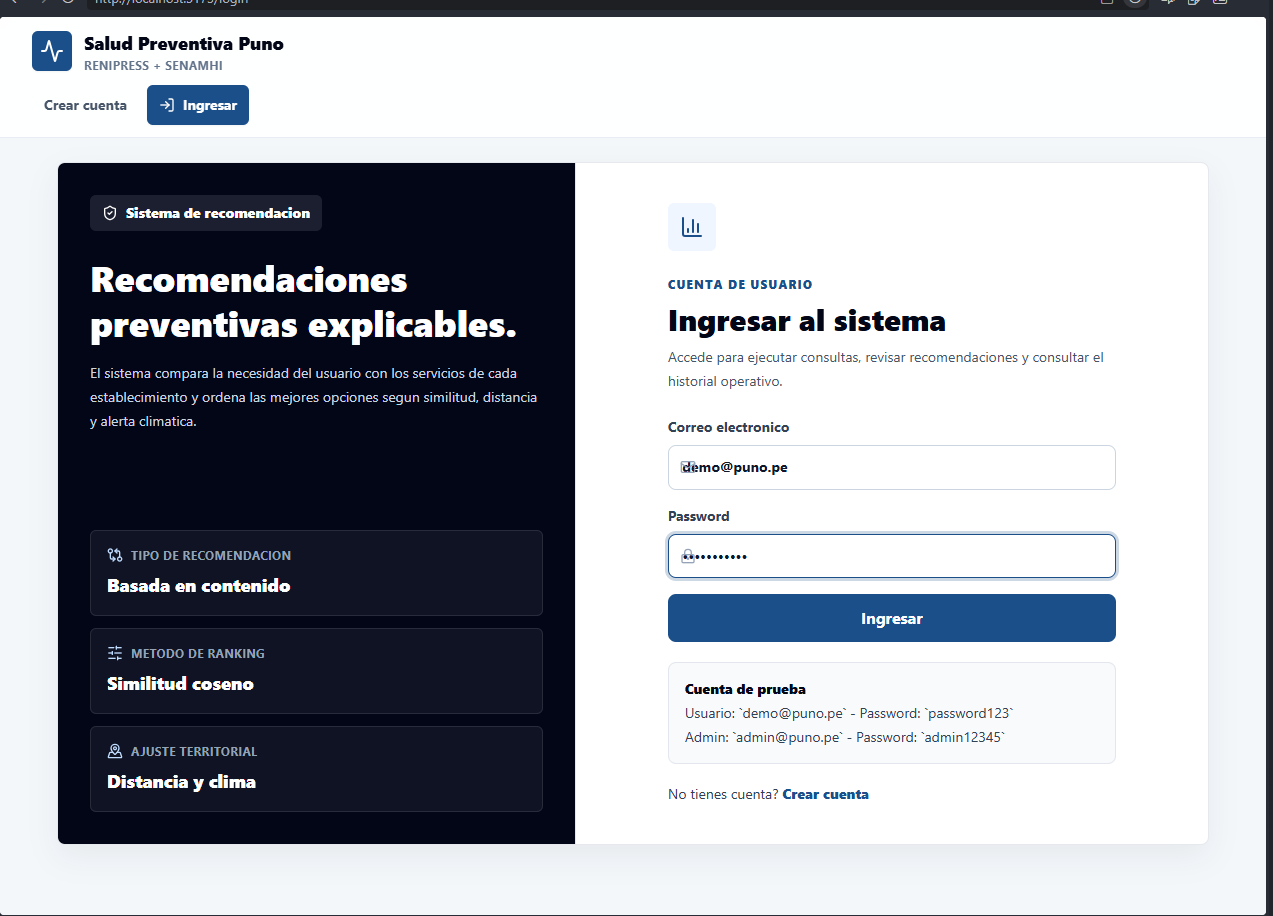
\includegraphics[width=0.92\textwidth]{login.png}
\caption{Pantalla de acceso con explicacion del enfoque de recomendacion.}
\label{fig:login}
\end{figure}

\begin{figure}[H]
\centering
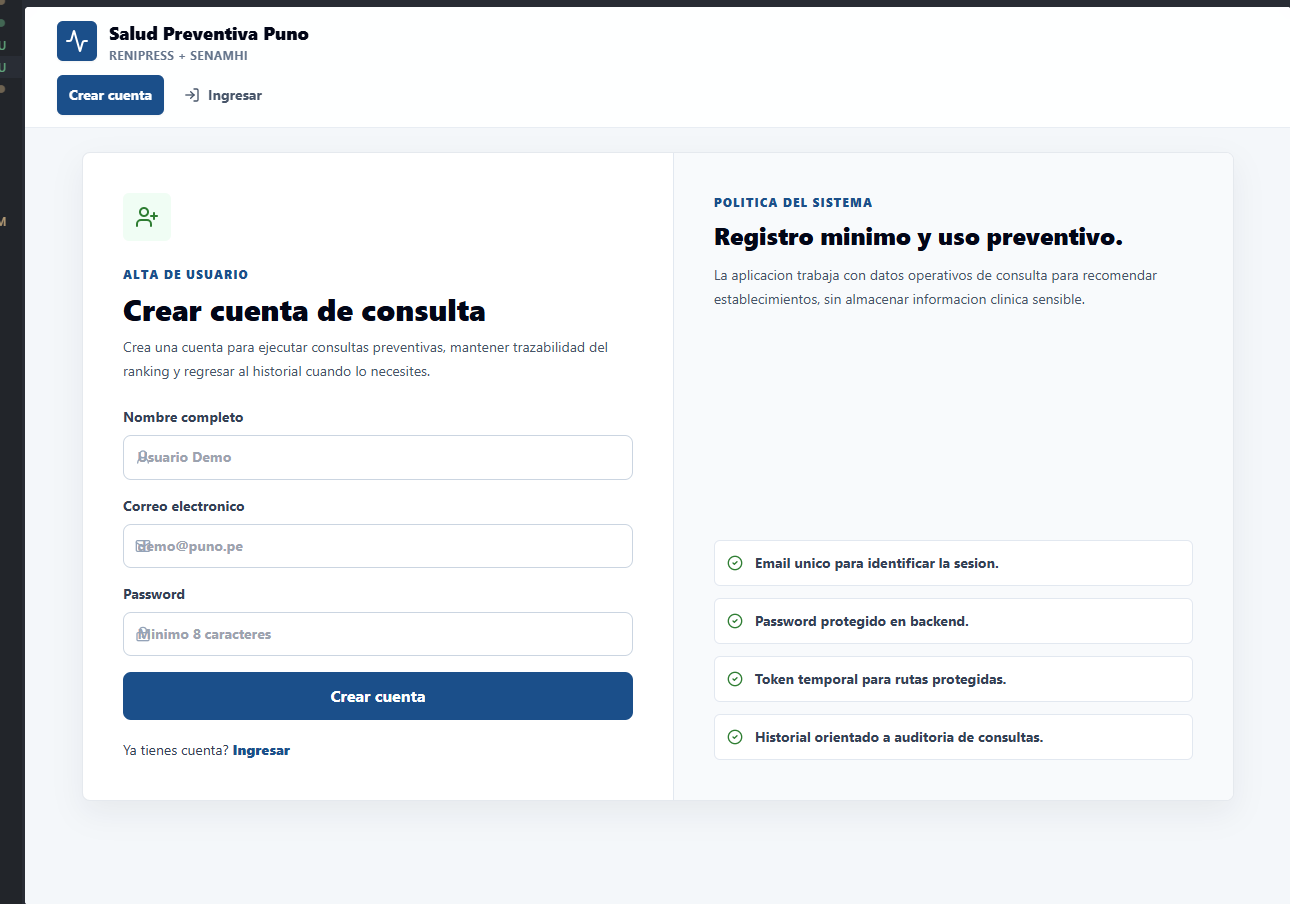
\includegraphics[width=0.92\textwidth]{crear_cuenta.png}
\caption{Pantalla de creacion de cuenta.}
\label{fig:registro}
\end{figure}

\begin{figure}[H]
\centering
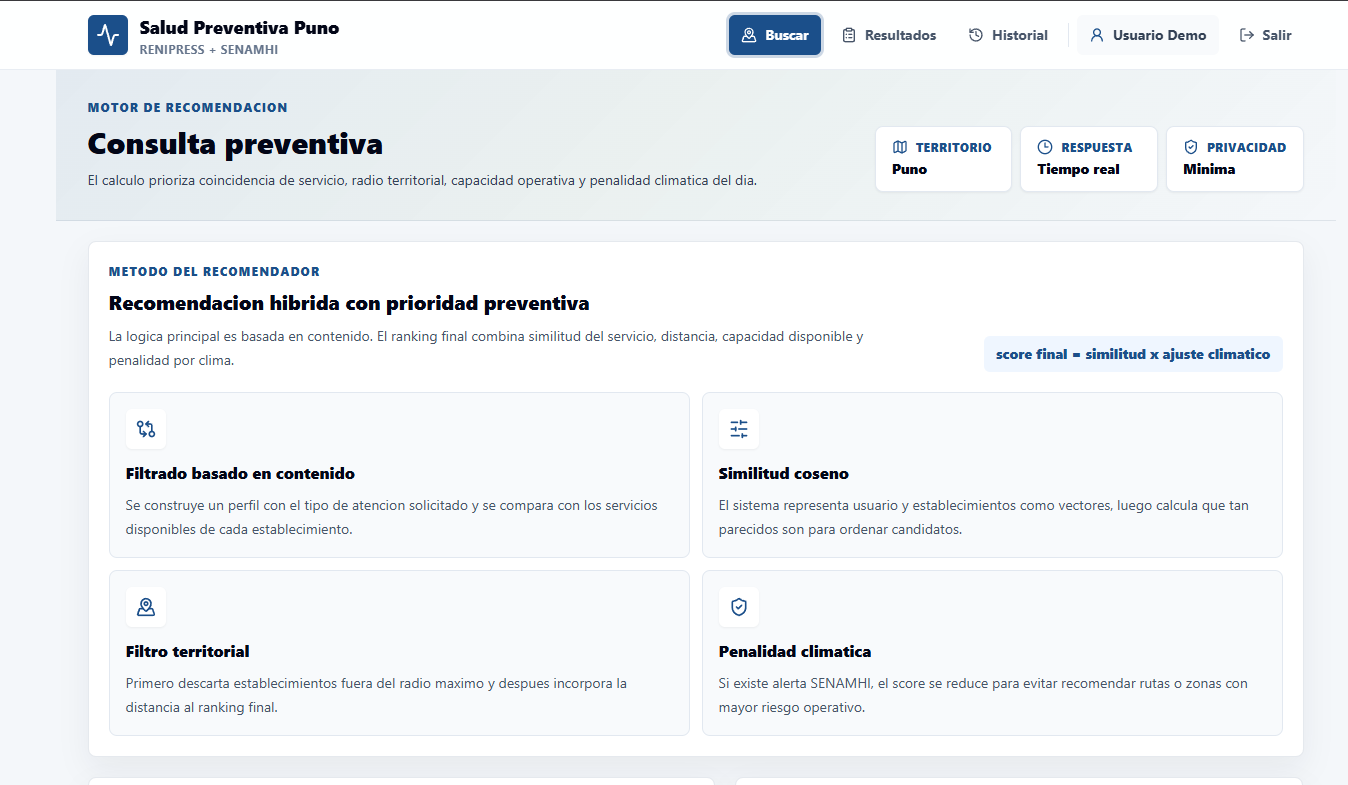
\includegraphics[width=0.92\textwidth]{inicio.png}
\caption{Pantalla de consulta preventiva.}
\label{fig:consulta}
\end{figure}

\begin{figure}[H]
\centering
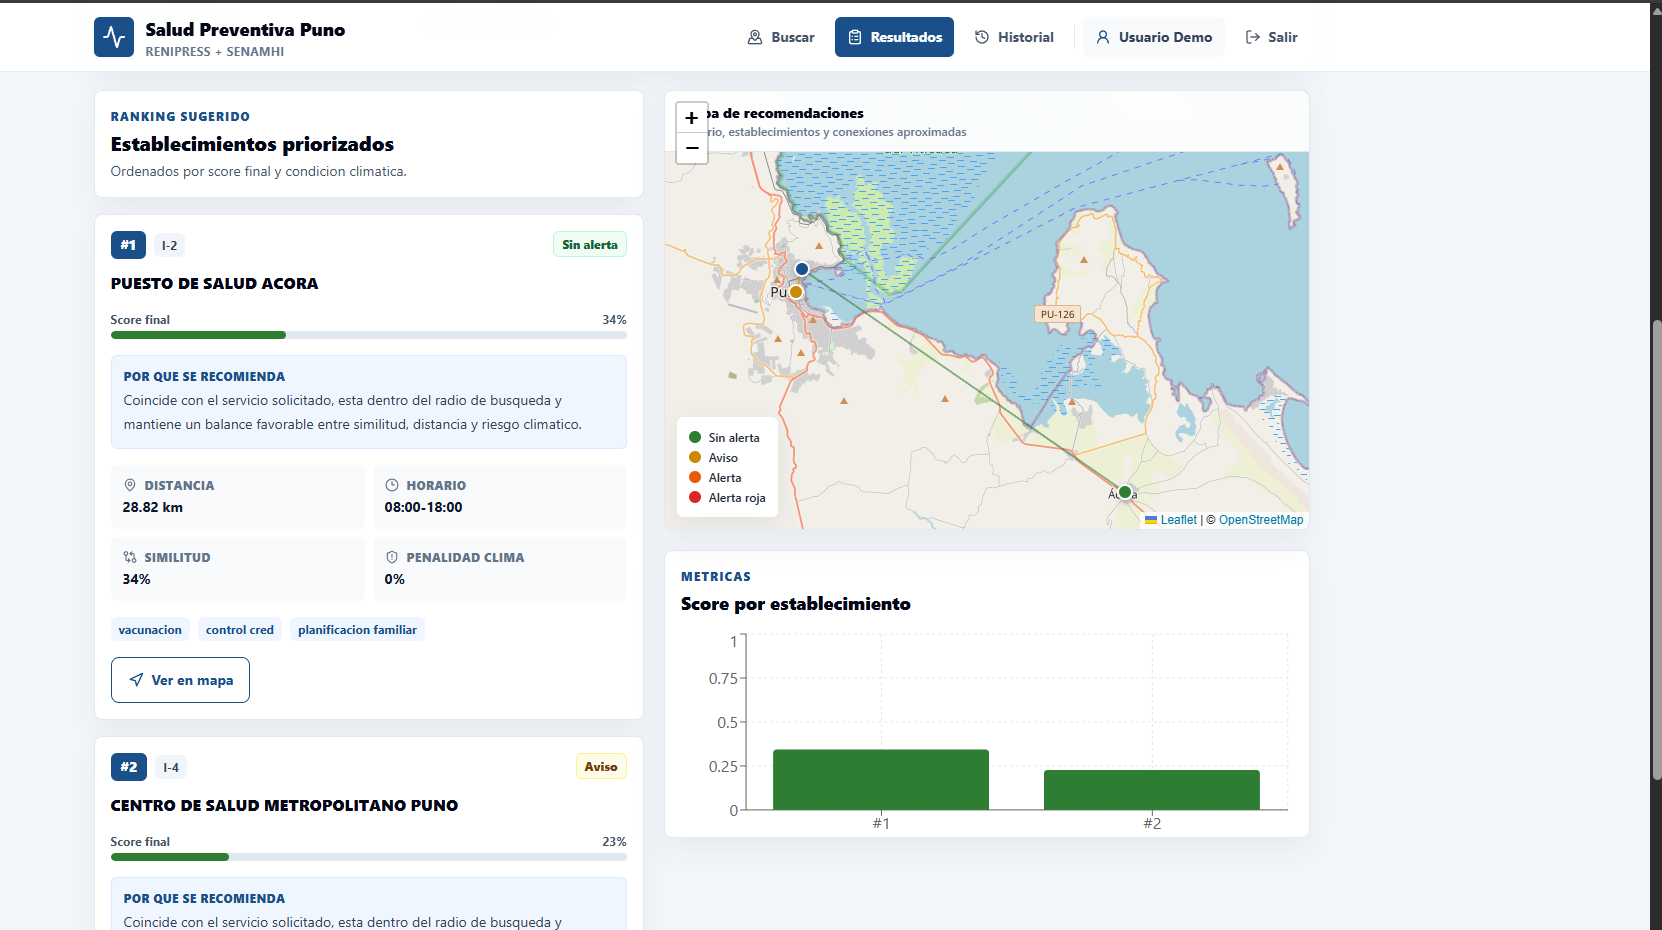
\includegraphics[width=0.92\textwidth]{luego_de_buscar.png}
\caption{Pantalla de resultados con ranking de centros recomendados.}
\label{fig:resultados}
\end{figure}

\begin{figure}[H]
\centering
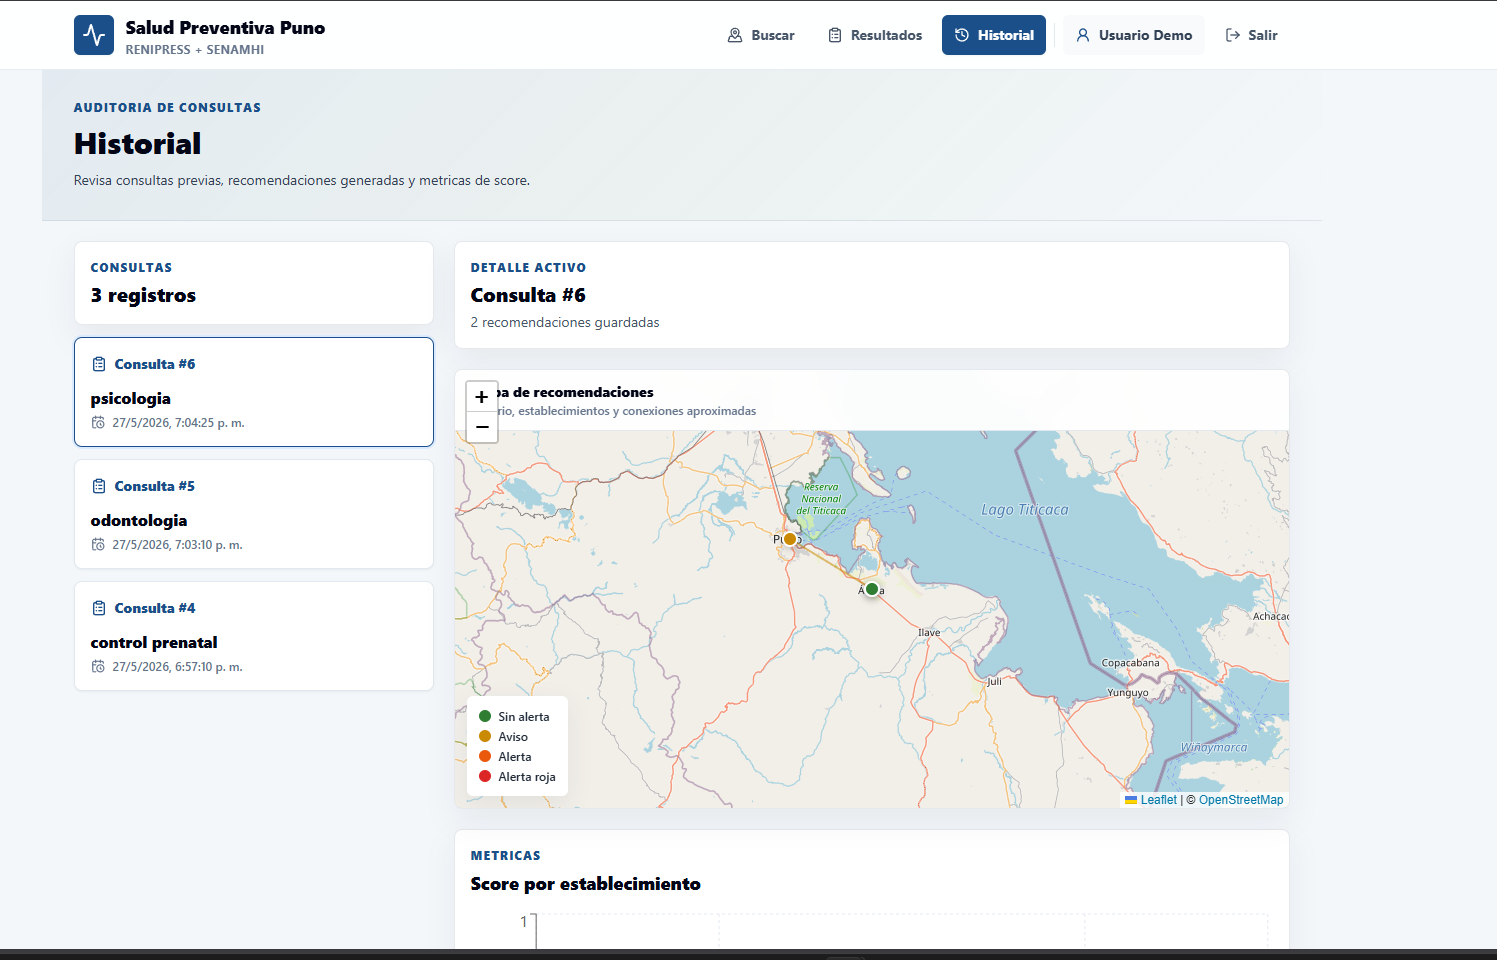
\includegraphics[width=0.92\textwidth]{historial.png}
\caption{Historial de consultas realizadas.}
\label{fig:historial}
\end{figure}

\subsection{Resultado del ranking}
El ranking generado permite comparar centros de salud de acuerdo con su relacion con la consulta. Un establecimiento sube en la lista cuando coincide mejor con el servicio solicitado y se encuentra dentro del radio definido. Por el contrario, un establecimiento puede bajar si presenta mayor distancia o alerta climatica.

\begin{figure}[H]
\centering
\begin{tikzpicture}
\begin{axis}[
    ybar,
    width=0.86\textwidth,
    height=7cm,
    bar width=16pt,
    ylabel={Score final referencial},
    xlabel={Rank},
    symbolic x coords={1,2,3,4,5},
    xtick=data,
    ymin=0,
    ymax=0.75,
    nodes near coords,
    grid=major,
    grid style={gray!15}
]
\addplot[fill=verdeSalud!75] coordinates {(1,0.61) (2,0.48) (3,0.43) (4,0.39) (5,0.25)};
\end{axis}
\end{tikzpicture}
\caption{Ejemplo de comportamiento descendente del score en Top-5.}
\label{fig:score}
\end{figure}

\subsection{Resultado de validacion}
El sistema fue probado localmente. El backend aprobo 13 pruebas automatizadas. El frontend compilo correctamente. Ademas, se verifico que la aplicacion responda en el navegador y que las rutas principales permitan completar el flujo de uso.

\begin{table}[H]
\centering
\caption{Evidencias de validacion.}
\label{tab:evidencias_validacion}
\begin{tabular}{p{5cm}p{7.5cm}}
\toprule
Evidencia & Descripcion \\
\midrule
Pruebas backend & 13 pruebas aprobadas. \\
Compilacion frontend & Construccion correcta del proyecto web. \\
Capturas & Registro visual del funcionamiento de pantallas. \\
Notebook & Evidencia del analisis y preparacion de datos. \\
Informe tecnico & Documento ampliado con fases, modelo y arquitectura. \\
\bottomrule
\end{tabular}
\end{table}

\subsection{Resultado del despliegue web}
Ademas de la ejecucion local, el proyecto fue publicado como aplicacion web. Este paso fue importante porque permite mostrar el sistema mediante enlaces publicos durante la sustentacion, sin tener que enviar todo el codigo por una carpeta comprimida o por Drive. La publicacion se organizo en tres partes: frontend en Vercel, backend en Render y base de datos PostgreSQL administrada en Render.

\begin{table}[H]
\centering
\caption{Recursos publicados del proyecto.}
\label{tab:recursos_publicados}
\small
\begin{tabular}{p{3.8cm}p{8.5cm}}
\toprule
Recurso & Enlace \\ 
\midrule
Repositorio GitHub & \url{https://github.com/tamoil-0/SistemasRecomendacion.git} \\
Aplicacion web & \url{https://sistemas-recomendacion.vercel.app} \\
API del sistema & \url{https://salud-preventiva-puno-api.onrender.com} \\
Documentacion de API & \url{https://salud-preventiva-puno-api.onrender.com/docs} \\
\bottomrule
\end{tabular}
\end{table}

El despliegue tambien permitio validar la integracion entre componentes. El frontend publicado consume el backend mediante la variable \texttt{VITE\_API\_URL}. El backend, a su vez, se conecta a PostgreSQL usando variables de entorno configuradas en Render. Para que la comunicacion entre ambos servicios funcione desde navegador, se configuro CORS con el dominio del frontend desplegado. Con ello, el login, registro, busqueda de recomendaciones e historial pueden ejecutarse desde la version publicada.

En el repositorio GitHub se dejo el codigo fuente necesario para reconstruir el sistema. Se excluyeron archivos generados o locales como entornos virtuales, \texttt{node\_modules/}, archivos \texttt{.env}, bases de datos SQLite locales y carpetas de compilacion. Esta organizacion facilita la revision del proyecto y evita subir dependencias innecesarias o informacion sensible.

\section{Discusion}
El proyecto demuestra que un sistema de recomendacion puede aplicarse a un problema regional y preventivo. A diferencia de los ejemplos habituales del curso, donde se recomiendan peliculas o productos, aqui se recomienda una alternativa de salud. Esto obliga a que el sistema sea mas cuidadoso en la forma de presentar sus resultados.

El enfoque basado en contenido fue una decision adecuada. Para aplicar filtrado colaborativo se necesitarian muchos usuarios, historiales de consultas, calificaciones o interacciones reales. Como el prototipo se encuentra en una etapa inicial, era mas razonable utilizar los atributos de los establecimientos. De esa manera, el sistema puede recomendar sin depender de una base historica extensa.

Otro punto importante es la explicabilidad. En un recomendador de entretenimiento, el usuario puede aceptar o ignorar una sugerencia sin mayor consecuencia. En cambio, en salud preventiva, aunque no se trate de una recomendacion clinica, el usuario necesita entender por que se le muestra un establecimiento. Por eso se incorporaron razones visibles, score, distancia, similitud y alerta climatica.

La inclusion del clima tambien aporta una diferencia frente a un recomendador simple. En la region Puno, la accesibilidad puede cambiar segun condiciones climaticas. Penalizar resultados con alerta permite que el ranking sea mas responsable. No elimina automaticamente un establecimiento, pero reduce su prioridad cuando existe mayor riesgo.

El trabajo tambien evidencio la importancia de la interfaz. Una aplicacion puede tener un modelo correcto, pero si la pantalla muestra informacion confusa o demasiado tecnica, el usuario no comprende el resultado. La mejora visual realizada permitio que el sistema se perciba mas formal, limpio y relacionado con el curso.

Finalmente, el despliegue en web aporto una validacion adicional. No solo se comprobo que el prototipo funcionara en la computadora de desarrollo, sino tambien que pudiera ejecutarse como sistema publicado, con frontend, API y base de datos conectados mediante servicios en la nube. Esto refuerza la presentacion del proyecto como prototipo funcional completo.

\subsection{Limitaciones}
La principal limitacion es que el prototipo trabaja con datos preparados para ejecucion local. Para una implementacion real seria necesario actualizar informacion desde fuentes oficiales, validar horarios, confirmar disponibilidad efectiva de servicios y revisar cambios en establecimientos.

Otra limitacion es la falta de retroalimentacion real de usuarios. El sistema todavia no aprende de preferencias acumuladas ni de visitas confirmadas. Si en el futuro se recopila ese tipo de informacion, podria evolucionar hacia un recomendador hibrido.

\subsection{Mejoras futuras}
Entre las mejoras futuras se proponen:

\begin{itemize}[leftmargin=*]
  \item Integrar datos oficiales actualizados de establecimientos.
  \item Mostrar fecha de actualizacion de servicios y alertas.
  \item Agregar confirmacion de disponibilidad o contacto del establecimiento.
  \item Recoger retroalimentacion del usuario despues de usar la recomendacion.
  \item Implementar un modelo hibrido cuando exista historial suficiente.
  \item Mejorar los indicadores visuales de explicacion del score.
\end{itemize}

\section{Conclusiones}
\begin{itemize}[leftmargin=*]
  \item Se desarrollo un prototipo funcional de sistema de recomendacion aplicado al dominio de salud preventiva en Puno.
  \item El proyecto cumple con los elementos principales del curso: usuarios, items, interacciones, atributos, ranking y evaluacion.
  \item El enfoque basado en contenido fue apropiado porque permite recomendar usando caracteristicas de los establecimientos sin requerir calificaciones historicas.
  \item La metodologia incluyo definicion del problema, preparacion de datos, analisis exploratorio, ajuste del modelo, desarrollo web y validacion.
  \item El sistema genera recomendaciones Top-N y presenta informacion suficiente para interpretar cada resultado.
  \item La interfaz fue mejorada para comunicar de forma formal el funcionamiento del recomendador y facilitar la sustentacion.
  \item El proyecto fue publicado en la web mediante Vercel y Render, por lo que puede ser revisado desde enlaces publicos.
  \item Las evidencias del notebook, capturas, pruebas e informes respaldan que el prototipo fue implementado de manera completa.
\end{itemize}

\section{Evidencias}
\subsection{Notebook}
El notebook del proyecto contiene el proceso de preparacion y analisis de datos. En el se revisa la informacion disponible, se realizan transformaciones y se valida la logica base del recomendador.

\begin{itemize}[leftmargin=*]
  \item Archivo: \texttt{notebook/sistema\_recomendacion\_salud\_puno.ipynb}
  \item Evidencia: analisis exploratorio, transformaciones, pruebas de recomendacion y soporte del modelo.
\end{itemize}

\subsection{Informe tecnico}
El informe tecnico desarrolla el proyecto con mayor detalle, incluyendo arquitectura, fases del prototipo, modelo, pruebas y anexos.

\begin{itemize}[leftmargin=*]
  \item Archivo fuente: \texttt{informe/informe\_tecnico.tex}
  \item Archivo compilado: \texttt{informe/informe\_tecnico.pdf}
\end{itemize}

\subsection{Repositorio y despliegue}
Como evidencia de publicacion, el proyecto cuenta con repositorio y servicios desplegados:

\begin{itemize}[leftmargin=*]
  \item Repositorio GitHub: \href{https://github.com/tamoil-0/SistemasRecomendacion.git}{github.com/tamoil-0/SistemasRecomendacion}.
  \item Frontend en Vercel: \href{https://sistemas-recomendacion.vercel.app}{sistemas-recomendacion.vercel.app}.
  \item Backend en Render: \href{https://salud-preventiva-puno-api.onrender.com}{salud-preventiva-puno-api.onrender.com}.
  \item Documentacion de API: \href{https://salud-preventiva-puno-api.onrender.com/docs}{salud-preventiva-puno-api.onrender.com/docs}.
\end{itemize}

\subsection{Capturas}
Las capturas se encuentran en la carpeta \texttt{capturas/}. Estas imagenes evidencian que el prototipo cuenta con interfaz funcional y pantallas completas.

\begin{table}[H]
\centering
\caption{Capturas usadas como evidencia.}
\label{tab:capturas}
\begin{tabular}{p{4cm}p{8cm}}
\toprule
Archivo & Evidencia \\
\midrule
landing.png & Presentacion general del sistema. \\
login.png & Acceso y explicacion del enfoque de recomendacion. \\
crear\_cuenta.png & Registro de usuarios. \\
inicio.png & Formulario de consulta preventiva. \\
luego\_de\_buscar.png & Ranking, mapa y resultados. \\
historial.png & Consultas realizadas anteriormente. \\
\bottomrule
\end{tabular}
\end{table}

\subsection{Sustentacion breve}
Para la sustentacion se recomienda seguir este orden:

\begin{enumerate}[leftmargin=*]
  \item Presentar el problema: necesidad de orientar consultas preventivas en Puno.
  \item Explicar el dominio: usuarios, establecimientos e interacciones.
  \item Describir el enfoque: recomendacion basada en contenido.
  \item Explicar como se preparo el modelo: datos, atributos, similitud, distancia y clima.
  \item Mostrar la aplicacion: login, busqueda, resultados e historial.
  \item Interpretar una recomendacion: servicio solicitado, distancia, score y alerta.
  \item Cerrar con conclusiones, limitaciones y mejoras futuras.
\end{enumerate}

\subsection{Resumen para exposicion}
El proyecto consiste en un sistema de recomendacion que orienta al usuario hacia centros de salud preventiva en Puno. El sistema usa un enfoque basado en contenido, porque compara la necesidad del usuario con las caracteristicas de los establecimientos. Considera servicio solicitado, ubicacion, distancia y alerta climatica. Como resultado, muestra un ranking Top-N con explicacion, mapa, puntajes e historial. El prototipo fue implementado como aplicacion web, validado con pruebas y documentado mediante notebook, capturas e informes.

\end{document}
